% Options for packages loaded elsewhere
\PassOptionsToPackage{unicode}{hyperref}
\PassOptionsToPackage{hyphens}{url}
\documentclass[
  ignorenonframetext,
]{beamer}
\newif\ifbibliography
\usepackage{pgfpages}
\setbeamertemplate{caption}[numbered]
\setbeamertemplate{caption label separator}{: }
\setbeamercolor{caption name}{fg=normal text.fg}
\beamertemplatenavigationsymbolsempty
% remove section numbering
\setbeamertemplate{part page}{
  \centering
  \begin{beamercolorbox}[sep=16pt,center]{part title}
    \usebeamerfont{part title}\insertpart\par
  \end{beamercolorbox}
}
\setbeamertemplate{section page}{
  \centering
  \begin{beamercolorbox}[sep=12pt,center]{section title}
    \usebeamerfont{section title}\insertsection\par
  \end{beamercolorbox}
}
\setbeamertemplate{subsection page}{
  \centering
  \begin{beamercolorbox}[sep=8pt,center]{subsection title}
    \usebeamerfont{subsection title}\insertsubsection\par
  \end{beamercolorbox}
}
% Prevent slide breaks in the middle of a paragraph
\widowpenalties 1 10000
\raggedbottom
\AtBeginPart{
  \frame{\partpage}
}
\AtBeginSection{
  \ifbibliography
  \else
    \frame{\sectionpage}
  \fi
}
\AtBeginSubsection{
  \frame{\subsectionpage}
}
\usepackage{iftex}
\ifPDFTeX
  \usepackage[T1]{fontenc}
  \usepackage[utf8]{inputenc}
  \usepackage{textcomp} % provide euro and other symbols
\else % if luatex or xetex
  \usepackage{unicode-math} % this also loads fontspec
  \defaultfontfeatures{Scale=MatchLowercase}
  \defaultfontfeatures[\rmfamily]{Ligatures=TeX,Scale=1}
\fi
\usepackage{lmodern}
\ifPDFTeX\else
  % xetex/luatex font selection
\fi
% Use upquote if available, for straight quotes in verbatim environments
\IfFileExists{upquote.sty}{\usepackage{upquote}}{}
\IfFileExists{microtype.sty}{% use microtype if available
  \usepackage[]{microtype}
  \UseMicrotypeSet[protrusion]{basicmath} % disable protrusion for tt fonts
}{}
\makeatletter
\@ifundefined{KOMAClassName}{% if non-KOMA class
  \IfFileExists{parskip.sty}{%
    \usepackage{parskip}
  }{% else
    \setlength{\parindent}{0pt}
    \setlength{\parskip}{6pt plus 2pt minus 1pt}}
}{% if KOMA class
  \KOMAoptions{parskip=half}}
\makeatother
\usepackage{longtable,booktabs,array}
\newcounter{none} % for unnumbered tables
\usepackage{calc} % for calculating minipage widths
\usepackage{caption}
% Make caption package work with longtable
\makeatletter
\def\fnum@table{\tablename~\thetable}
\makeatother
\usepackage{graphicx}
\makeatletter
\newsavebox\pandoc@box
\newcommand*\pandocbounded[1]{% scales image to fit in text height/width
  \sbox\pandoc@box{#1}%
  \Gscale@div\@tempa{\textheight}{\dimexpr\ht\pandoc@box+\dp\pandoc@box\relax}%
  \Gscale@div\@tempb{\linewidth}{\wd\pandoc@box}%
  \ifdim\@tempb\p@<\@tempa\p@\let\@tempa\@tempb\fi% select the smaller of both
  \ifdim\@tempa\p@<\p@\scalebox{\@tempa}{\usebox\pandoc@box}%
  \else\usebox{\pandoc@box}%
  \fi%
}
% Set default figure placement to htbp
\def\fps@figure{htbp}
\makeatother
\setlength{\emergencystretch}{3em} % prevent overfull lines
\providecommand{\tightlist}{%
  \setlength{\itemsep}{0pt}\setlength{\parskip}{0pt}}
\usepackage{bookmark}
\IfFileExists{xurl.sty}{\usepackage{xurl}}{} % add URL line breaks if available
\urlstyle{same}
\hypersetup{
  pdftitle={Case Systems and Grammatical Relations},
  hidelinks,
  pdfcreator={LaTeX via pandoc}}

\title{\texorpdfstring{Case Systems and Grammatical
Relations}{Case Systems and Grammatical Relations}}
\author{\texorpdfstring{}{}}
\date{}

\begin{document}
\frame{\titlepage}

\section{Case Systems, Grammatical Relations, and Alignment
Typology}\label{sec:case-systems}

\begin{frame}{Historical Foundations: From Pāṇini to Jakobson, Fillmore,
and Mel'čuk}
\protect\phantomsection\label{historical-foundations-from-pux101ux1e47ini-to-jakobson-fillmore-and-melux10duk}
The formal study of grammatical case begins with the Sanskrit grammarian
Pāṇini (c.~4th-5th century BCE), whose \emph{Aṣṭādhyāyī} formalized the
\emph{Kāraka} theory --- a semantic system of deep roles (e.g., agent,
patient) linking nouns to verbs in Sanskrit grammar. Etymologically
meaning ``that which brings about'' an action, the Kāraka system
expresses world knowledge through rigorous mappings from deep semantic
relations to phonological representations via case endings. As later
structuralists noted, ``Semantics and phonetics have been the basis of
all linguistic analysis in the Sanskritic tradition\ldots{} providing
steps for semantic interpretation through carefully crafted
morpho-syntactic procedures'' {[}-@jha2021sanskrit;
-@kak1987paninian{]}.

This profound insight---that a finite set of relational roles underlies
the infinite variety of sentences---was resurrected in modern
linguistics by Charles Fillmore's seminal ``The Case for Case'' (1968),
which explicitly acknowledged its Pāṇinian inheritance while proposing
\emph{deep cases} (Agentive, Objective, Dative) as universal semantic
primitives {[}-@fillmore1968case{]}. In parallel, structuralist
formalisms pioneered by Roman Jakobson in \emph{Morphologic Inquiry into
Slavic Declension} (1958) and Louis Hjelmslev in \emph{La catégorie des
cas} (1935) treated case not merely as semantic markers, but as formal
systems of paradigmatic and syntagmatic oppositions --- treating cases
as bundles of structural features rather than isolated labels
{[}-@jakobson1958morphologic; -@hjelmslev1935categorie{]}.

Fillmore's deep cases were precursors to modern \emph{thematic role}
theory. Dowty {[}-@dowty1991thematic{]} refined the approach by
decomposing thematic roles into clusters of sentential entailments,
yielding two \emph{proto-roles}: the Proto-Agent (characterized by
volitional involvement, sentience, causation, movement) and the
Proto-Patient (characterized by undergoing change of state, incremental
theme, causal affectedness, stationary relative to another participant).
This decomposition is significant for our categorical formalization
because it replaces a discrete role inventory with a \emph{graded}
structure---morphisms in our case category can carry weights reflecting
the degree to which a noun phrase satisfies proto-role entailments.

Between Pāṇini and Fillmore, the structuralist and functionalist
traditions of the early 20th century---particularly those rooted in
Russian and Slavic linguistics---laid essential groundwork. Roman
Jakobson's 1936 formalization of the Russian six-case system
(nominative, genitive, dative, accusative, instrumental, prepositional)
employed binary distinctive features (e.g., {[}±directional{]},
{[}±peripheral{]}), treating case oppositions analogously to
phonological oppositions and revealing that morphological paradigms
possess an internal algebraic structure. The Prague Linguistic Circle,
led by Nikolai Trubetzkoy and Sergej Karcevskij alongside Jakobson,
extended this functionalist analysis to Czech and other Slavic
languages, emphasizing \emph{markedness} hierarchies and the
communicative load of case distinctions---insights that anticipate the
weighted morphisms of our categorical framework. Louis Hjelmslev's
glossematics (1930s--1940s), though Danish in origin, resonated deeply
within Slavic formalism by positing case as a purely relational category
within a sign/content dichotomy, prefiguring Fillmore's abstractions
from surface morphology. Igor Mel'čuk's Meaning-Text Theory
(1970s--present) models Russian case assignment through deep syntactic
actants mapped to surface cases via dependency trees, providing a
computationally explicit formalization that bridges the gap between
Fillmore's semantic roles and contemporary distributional semantics.
\end{frame}

\begin{frame}{The Cross-Linguistic Typological Landscape}
\protect\phantomsection\label{the-cross-linguistic-typological-landscape}
Contemporary typological work reveals that the world's languages realize
case systems according to a small number of \emph{alignment
types}---systematic patterns governing how the core arguments of
transitive and intransitive clauses are grouped {[}@polinsky2015case;
@blake2001grammatical; @haspelmath2009universality{]}.

\begin{block}{Core Argument Roles}
\protect\phantomsection\label{core-argument-roles}
The cross-linguistic comparison rests on three primitives:

{\def\LTcaptype{none} % do not increment counter
\begin{longtable}[]{@{}
  >{\centering\arraybackslash}p{(\linewidth - 4\tabcolsep) * \real{0.3571}}
  >{\raggedright\arraybackslash}p{(\linewidth - 4\tabcolsep) * \real{0.3571}}
  >{\raggedright\arraybackslash}p{(\linewidth - 4\tabcolsep) * \real{0.2857}}@{}}
\toprule\noalign{}
\begin{minipage}[b]{\linewidth}\centering
Symbol
\end{minipage} & \begin{minipage}[b]{\linewidth}\raggedright
Role
\end{minipage} & \begin{minipage}[b]{\linewidth}\raggedright
Definition
\end{minipage} \\
\midrule\noalign{}
\endhead
\textbf{S} & Sole argument of intransitive & ``The child
\textbf{sleeps}'' \\
\textbf{A} & Agent-like argument of transitive & ``\textbf{The child}
broke the vase'' \\
\textbf{P} & Patient-like argument of transitive & ``The child broke
\textbf{the vase}'' \\
\bottomrule\noalign{}
\end{longtable}
}
\end{block}

\begin{block}{Alignment Systems}
\protect\phantomsection\label{alignment-systems}
The key insight from typological research is that languages differ in
how they \emph{group} these three roles for purposes of case marking,
agreement, and other grammatical processes:

{\def\LTcaptype{none} % do not increment counter
\begin{longtable}[]{@{}
  >{\raggedright\arraybackslash}p{(\linewidth - 4\tabcolsep) * \real{0.3333}}
  >{\raggedright\arraybackslash}p{(\linewidth - 4\tabcolsep) * \real{0.3333}}
  >{\raggedright\arraybackslash}p{(\linewidth - 4\tabcolsep) * \real{0.3333}}@{}}
\toprule\noalign{}
\begin{minipage}[b]{\linewidth}\raggedright
Alignment
\end{minipage} & \begin{minipage}[b]{\linewidth}\raggedright
Grouping
\end{minipage} & \begin{minipage}[b]{\linewidth}\raggedright
Exemplar Languages
\end{minipage} \\
\midrule\noalign{}
\endhead
\textbf{Nominative--Accusative} & S = A \(\neq\) P & English, Latin,
Finnish, Russian \\
\textbf{Ergative--Absolutive} & S = P \(\neq\) A & Basque, Dyirbal,
Georgian (partly) \\
\textbf{Active--Stative} & S splits by agentivity & Lakhota, Guaraní,
Eastern Pomo \\
\textbf{Tripartite} & S \(\neq\) A \(\neq\) P & Nez Perce, some
Australian languages \\
\textbf{Fluid-S} & S marking varies by context & Bats (NE Caucasian),
Acehnese \\
\bottomrule\noalign{}
\end{longtable}
}

Claassen {[}-@claassen2025alignment{]} provides a comprehensive survey
of the explanatory frameworks proposed for alignment diversity, arguing
that no single factor (processing efficiency, disambiguation, discourse
pragmatics) suffices---a conclusion that motivates our multi-dimensional
categorical formalization. Wu {[}-@wu2024amis{]} offers a detailed case
study of Amis (Austronesian), demonstrating how verb classification,
case marking, and grammatical relations interact in a language that
defies simple alignment classification.
\end{block}

\begin{block}{Extended Case Inventories and the CEREBRUM Framework}
\protect\phantomsection\label{extended-case-inventories-and-the-cerebrum-framework}
Beyond the three core arguments, languages distinguish a rich inventory
of oblique cases. Our formalization follows the CEREBRUM framework
{[}@friedman2024cerebrum{]} in adopting eight fundamental cases:

{\def\LTcaptype{none} % do not increment counter
\begin{longtable}[]{@{}
  >{\raggedright\arraybackslash}p{(\linewidth - 6\tabcolsep) * \real{0.2353}}
  >{\centering\arraybackslash}p{(\linewidth - 6\tabcolsep) * \real{0.2941}}
  >{\raggedright\arraybackslash}p{(\linewidth - 6\tabcolsep) * \real{0.2353}}
  >{\raggedright\arraybackslash}p{(\linewidth - 6\tabcolsep) * \real{0.2353}}@{}}
\toprule\noalign{}
\begin{minipage}[b]{\linewidth}\raggedright
Case
\end{minipage} & \begin{minipage}[b]{\linewidth}\centering
Abbreviation
\end{minipage} & \begin{minipage}[b]{\linewidth}\raggedright
Semantic Core
\end{minipage} & \begin{minipage}[b]{\linewidth}\raggedright
Syntactic Prototype
\end{minipage} \\
\midrule\noalign{}
\endhead
Nominative & NOM & Agent / experiencer & Intransitive subject,
transitive agent \\
Accusative & ACC & Patient / theme & Direct object, incremental theme \\
Genitive & GEN & Possessor / source & Possessive modifier, partitive \\
Dative & DAT & Recipient / goal & Indirect object, beneficiary \\
Instrumental & INS & Instrument / means & Adverbial of means \\
Locative & LOC & Location / context & Spatial/temporal ground \\
Ablative & ABL & Origin / cause & Source of motion, causal adjunct \\
Vocative & VOC & Addressee & Direct address \\
\bottomrule\noalign{}
\end{longtable}
}
\end{block}
\end{frame}

\begin{frame}[fragile]{Categorical Formalization of Case Systems}
\protect\phantomsection\label{categorical-formalization-of-case-systems}
\begin{block}{Case Categories as Directed Graphs}
\protect\phantomsection\label{case-categories-as-directed-graphs}
We define a \textbf{case category} \(\mathcal{C}\) as a small category
where:

\begin{itemize}
\tightlist
\item
  \textbf{Objects} are case roles (NOM, ACC, GEN, DAT, INS, LOC, ABL,
  VOC)
\item
  \textbf{Morphisms} are grammatical relations between roles (e.g.,
  ``transitive action'': NOM → ACC)
\item
  \textbf{Identity morphisms} represent the reflexive relation of each
  case role to itself
\item
  \textbf{Composition} models the transitivity of grammatical
  dependencies
\end{itemize}

This formalization is implemented in our \texttt{CaseCategory} class,
which uses a directed graph (via NetworkX) as the underlying
representation. Each object carries its role enum and optional
morphosyntactic features; each morphism carries a relation label and an
enriched weight \(w \in [0,1]\). \autoref{fig:case-standard} shows the
full eight-case standard category.

\begin{figure}
\centering
\pandocbounded{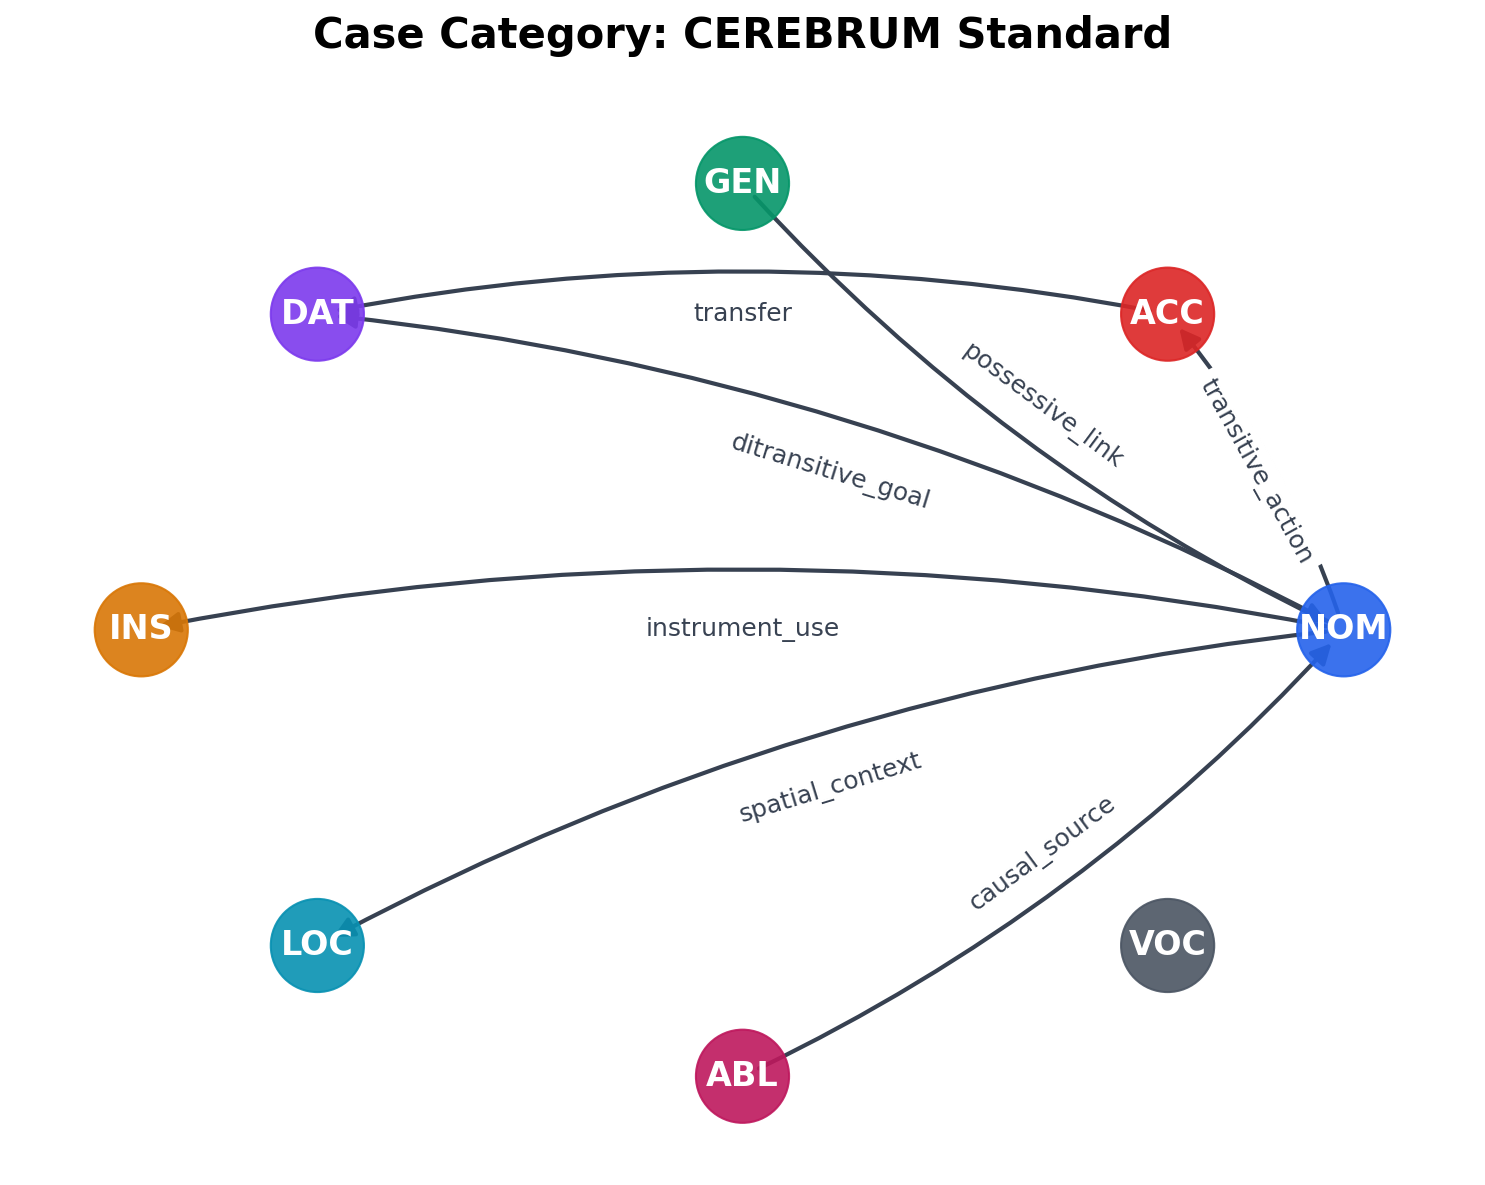
\includegraphics[keepaspectratio,alt={The standard linguistic case category with eight case roles (NOM, ACC, GEN, DAT, INS, LOC, ABL, VOC) and directed morphisms representing grammatical relations between them. Edge labels encode relation types (e.g., transitive action, possession, spatial grounding), and edge weights in the interval zero to one reflect proto-role satisfaction. Generated from the CaseCategory class.}]{../figures/case_category_standard.png}}
\caption{The standard linguistic case category with eight case roles
(NOM, ACC, GEN, DAT, INS, LOC, ABL, VOC) and directed morphisms
representing grammatical relations between them. Edge labels encode
relation types (e.g., transitive action, possession, spatial grounding),
and edge weights in the interval zero to one reflect proto-role
satisfaction. Generated from the CaseCategory
class.}\label{fig:case-standard}
\end{figure}
\end{block}

\begin{block}{Alignment Functors Between Case Categories}
\protect\phantomsection\label{alignment-functors-between-case-categories}
An \textbf{alignment functor} \(F: \mathcal{U} \to \mathcal{L}\) maps a
universal (maximal) case category \(\mathcal{U}\) to a language-specific
category \(\mathcal{L}\) by collapsing objects that a particular
language treats as equivalent. For example, in an accusative language,
the functor merges S and A into a single NOM role while keeping P as a
distinct ACC role: \(F(\text{S}) = F(\text{A}) = \text{NOM}\),
\(F(\text{P}) = \text{ACC}\).

This functor is:

\begin{itemize}
\tightlist
\item
  \textbf{Surjective on objects}: every case in the target language is
  the image of some universal role
\item
  \textbf{Structure-preserving}: grammatical relations in
  \(\mathcal{U}\) map to grammatical relations in \(\mathcal{L}\)
\item
  \textbf{Non-identity when alignment differs}: the kernel of \(F\) (the
  set of objects mapped to the same target) characterizes the alignment
  type
\end{itemize}

The alignment functor provides a formal account of neutralization: two
semantically distinct roles (S vs.~A) receive the same morphological
treatment because the functor maps them to the same object.
\autoref{fig:alignment} shows three alignment systems rendered from our
\texttt{CaseCategory} implementation.

\begin{figure}
\centering
\pandocbounded{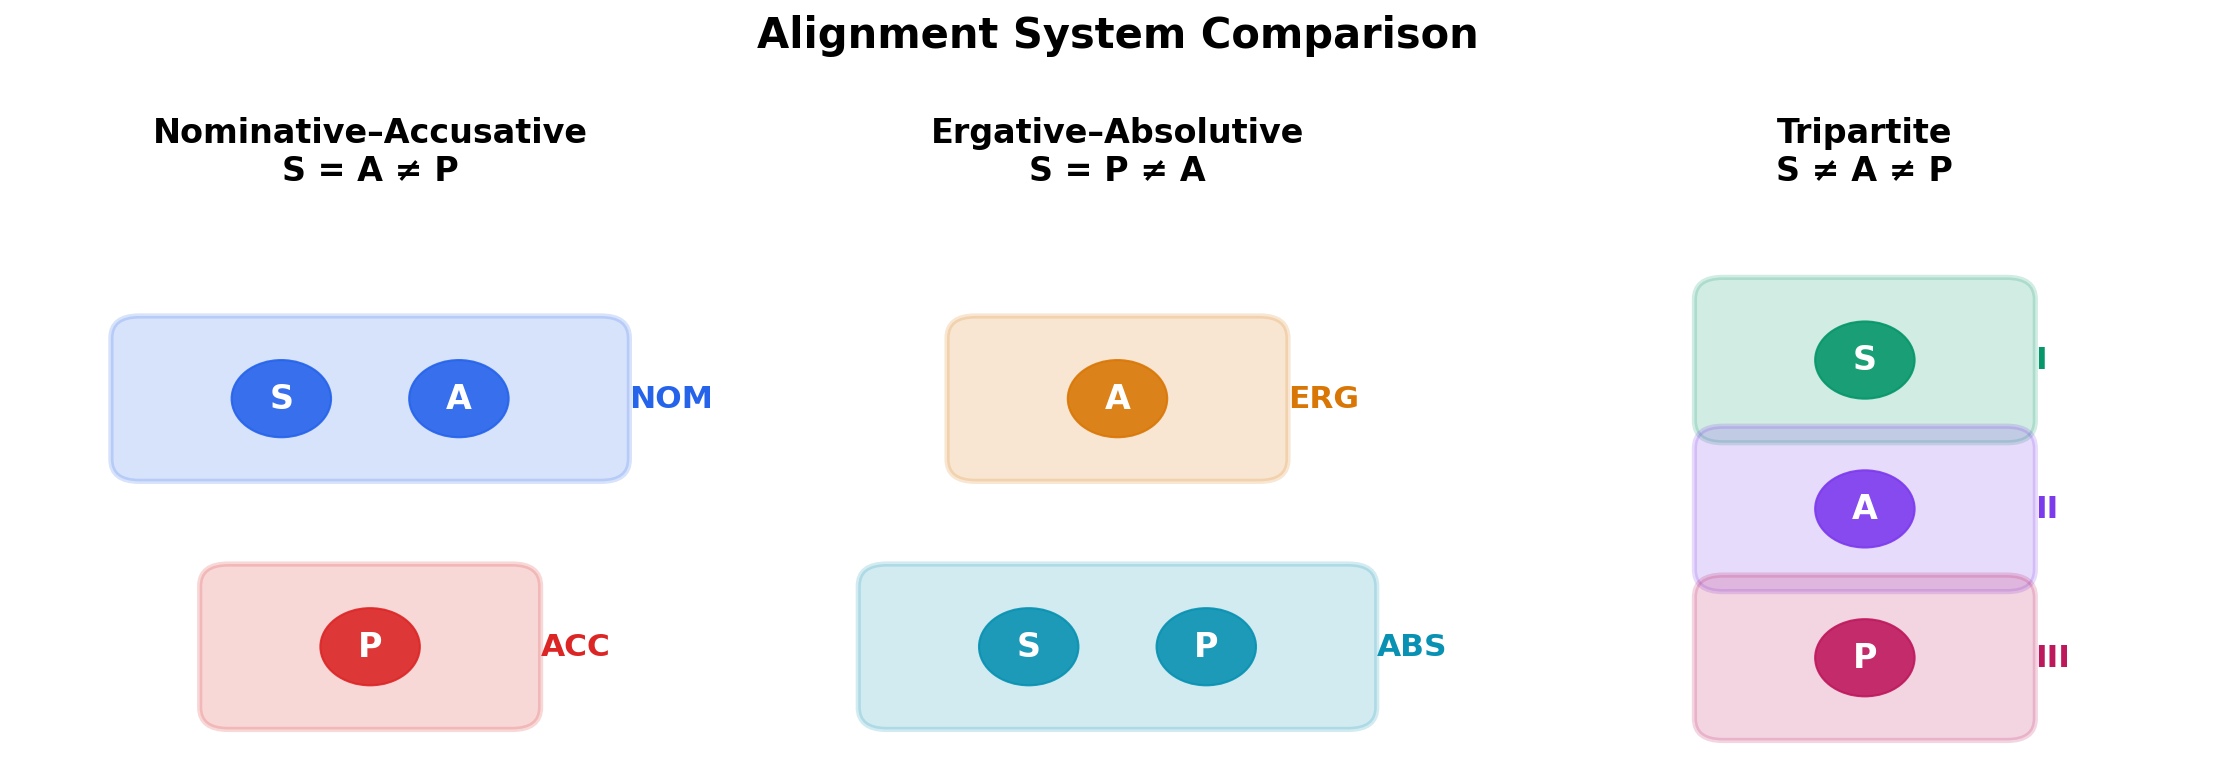
\includegraphics[keepaspectratio,alt={Side-by-side comparison of three alignment systems---Nominative-Accusative, Ergative-Absolutive, and Tripartite---showing how each alignment type groups the three core arguments (S, A, P) into distinct morphological categories. Color-coded nodes indicate case role identity; shared colors reveal the S=A or S=P neutralizations that define each alignment.}]{../figures/alignment_comparison.png}}
\caption{Side-by-side comparison of three alignment
systems---Nominative-Accusative, Ergative-Absolutive, and
Tripartite---showing how each alignment type groups the three core
arguments (S, A, P) into distinct morphological categories. Color-coded
nodes indicate case role identity; shared colors reveal the S=A or S=P
neutralizations that define each alignment.}\label{fig:alignment}
\end{figure}

\begin{figure}
\centering
\pandocbounded{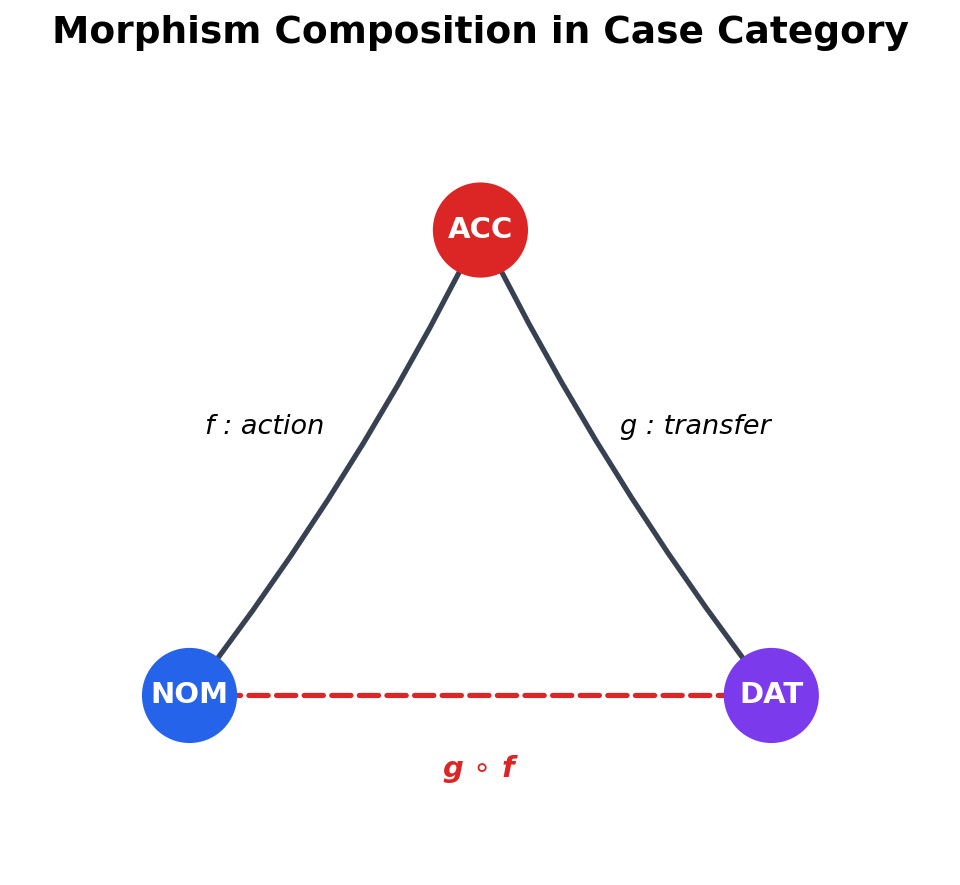
\includegraphics[keepaspectratio,alt={The categorical composition triangle: morphism f (transitive action, NOM to ACC) and morphism g (transfer, ACC to DAT) compose to yield g after f (NOM to DAT), illustrating how grammatical dependencies chain transitively through intermediate case roles. The commutativity of this triangle encodes that indirect object assignment factors through the direct object.}]{../figures/composition_triangle.png}}
\caption{The categorical composition triangle: morphism f (transitive
action, NOM to ACC) and morphism g (transfer, ACC to DAT) compose to
yield g after f (NOM to DAT), illustrating how grammatical dependencies
chain transitively through intermediate case roles. The commutativity of
this triangle encodes that indirect object assignment factors through
the direct object.}\label{fig:composition}
\end{figure}
\end{block}

\begin{block}{Enriched Morphisms, Proto-Roles, and Graded Structure}
\protect\phantomsection\label{enriched-morphisms-proto-roles-and-graded-structure}
Following Dowty {[}-@dowty1991thematic{]}, we equip morphisms with
weights in \([0,1]\) that encode the degree of proto-role satisfaction.
A morphism \(f: \text{NOM} \to \text{ACC}\) with weight \(w = 0.9\)
indicates a strong transitive action (clear agent acting on clear
patient), while \(w = 0.4\) might indicate an experiencer construction
(``The child fears the dark'') where the nominative argument only weakly
satisfies Proto-Agent entailments.

Composition of enriched morphisms multiplies weights:
\[w(g \circ f) = w(g) \cdot w(f) \tag{2.1}\]

This multiplicative composition reflects the intuition that grammatical
dependencies attenuate as they chain through intermediate roles.
\autoref{fig:composition} illustrates the categorical composition of two
morphisms through an intermediate case role. The resulting structure is
a category enriched over \(([0,1], \cdot, 1)\)---a connection we develop
fully in \autoref{sec:enriched-categories}.
\end{block}
\end{frame}

\end{document}
